\documentclass[tikz,border=2pt]{standalone}
\usepackage{newpxtext,newpxmath}
\definecolor{curve}{HTML}{1f6fb2}
\definecolor{accent}{HTML}{c0392b}
\definecolor{polygon}{HTML}{555555}
\definecolor{muted}{HTML}{dfe6ee}
\begin{document}
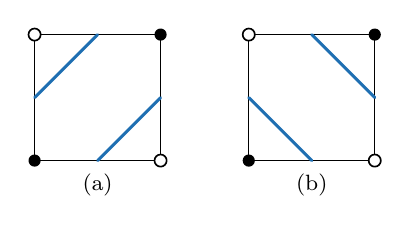
\begin{tikzpicture}[
  x=1.6cm, y=1.6cm,
  line cap=round, line join=round,
  every node/.style={font=\footnotesize, inner sep=1.5pt},
  curve/.style={draw=curve, line width=1.1pt},
  second/.style={draw=accent, line width=1.1pt},
  polygon/.style={line width=0.5pt, dash pattern=on 2.5pt off 2pt},
  construction/.style={draw=accent, line width=0.5pt},
  axis/.style={line width=0.45pt, draw=black!80, >=stealth},
  ctrl/.style={circle, fill=white, line width=0.6pt, minimum size=4pt, inner sep=0pt},
]
\draw[line width=0.5pt] (0,0) rectangle (1,1);
\draw[curve] (0.5000,0.0000) .. controls (0.6667,0.1667) and (0.8333,0.3333) .. (1.0000,0.5000);
\draw[curve] (0.5000,1.0000) .. controls (0.3333,0.8333) and (0.1667,0.6667) .. (0.0000,0.5000);
\fill[black] (0,0) circle (2.2pt);
\fill[black] (1,1) circle (2.2pt);
\node[ctrl, draw=black, minimum size=4.4pt] at (1,0) {};
\node[ctrl, draw=black, minimum size=4.4pt] at (0,1) {};
\node[below=3pt] at (0.5,0) {(a)};
\draw[line width=0.5pt] (1.7,0) rectangle (2.7,1);
\draw[curve] (2.2000,0.0000) .. controls (2.0333,0.1667) and (1.8667,0.3333) .. (1.7000,0.5000);
\draw[curve] (2.7000,0.5000) .. controls (2.5333,0.6667) and (2.3667,0.8333) .. (2.2000,1.0000);
\fill[black] (1.7,0) circle (2.2pt);
\fill[black] (2.7,1) circle (2.2pt);
\node[ctrl, draw=black, minimum size=4.4pt] at (2.7,0) {};
\node[ctrl, draw=black, minimum size=4.4pt] at (1.7,1) {};
\node[below=3pt] at (2.2,0) {(b)};
\end{tikzpicture}
\end{document}
